\begin{figure*}[t]
\vskip -0.2in
\centering
\begin{subfigure}[b]{0.5\textwidth}
  \centering
  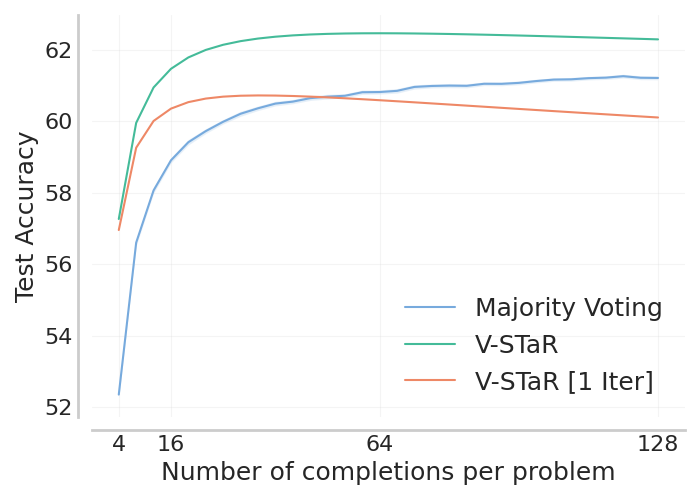
\includegraphics[scale=0.39]{icml2023/figs/maj_vs_ver_colm.png}
  % \caption{Test accuracy of 7B V-STaR compared to \vstar{}[1 Iter] and majority voting~\citep{DBLP:conf/iclr/0002WSLCNCZ23} across different numbers of candidate solutions generated on GSM8K. We subsample candidate solutions from $N=1000$ generations. V-STaR can rank over a reasonably large number of candidate solutions. We compute 95\% confidence interval for majority voting using 256 trials.}
    
\end{subfigure}%
\begin{subfigure}[b]{0.5\textwidth}
  \centering
  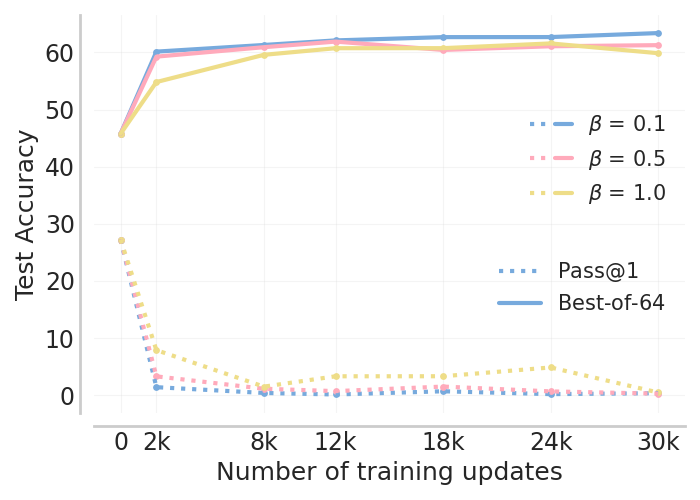
\includegraphics[scale=0.39]{icml2023/figs/ver_vs_gen_colm.png}
  % \caption{Comparing DPO-based generator and verifier for \vstar{} 7B, measured by Pass$@1$ and Verifier$@64$ respectively on GSM8K. Verifier$@64$ accuracy rises significantly while the generation ability of DPO verifier degrades with only 2k training steps.}
    
\end{subfigure}%
\caption{\textbf{Left:} \textbf{Best-of-k test accuracy} of 7B V-STaR compared to \vstar{}[1 Iter] and self-consistency~\citep{DBLP:conf/iclr/0002WSLCNCZ23} across different numbers of candidate solutions generated on GSM8K. We subsample  solutions from $N=1000$ generations. V-STaR can rank over a reasonably large number of candidate solutions. We compute 95\% CIs for self-consistency using 256 trials. \textbf{Right: Comparing DPO-based generator and verifier} for \vstar{} 7B, measured by Pass$@1$ and Best-of-$64$ respectively on GSM8K. Best-of-$64$ accuracy rises significantly while the generation ability of DPO verifier degrades with only 2k updates.}
% \label{fig:ver_at_k}
% \vskip 0.2in

\label{fig:ver_vs_maj}
\label{fig:ver_as_gen}
\end{figure*}